% This file was generated by qzm-view_test on Mon, 26 Sep 2011 20:37:16 -0700


%\documentclass{exam}            % w/ answers
\documentclass[noanswers]{exam}  % w/o answers

\usepackage{multicol}
\usepackage{ulem}
\usepackage{graphicx}
\usepackage{amsmath}

\parindent=0pt
%\usepackage{graphicx}

\begin{document}


% choose one or the other,
% or leave configured by \documentclass
\printanswers
%\noprintanswers


\begin{tabular}{l r}
Name: \uline{\hspace{200pt}} \hspace{160pt} & (no class) \\
      & (no term) \\
      & (testing image example) \\
\end{tabular}


\vspace{10pt}

This test shows how a problem can include an image.

\vspace{5pt}

\begin{questions}

\question Calculate the current through the voltage source and the resistor.

\vspace{0.2in} % add some space above the image
\begin{center}
%\begin{figure}[!hbtp]
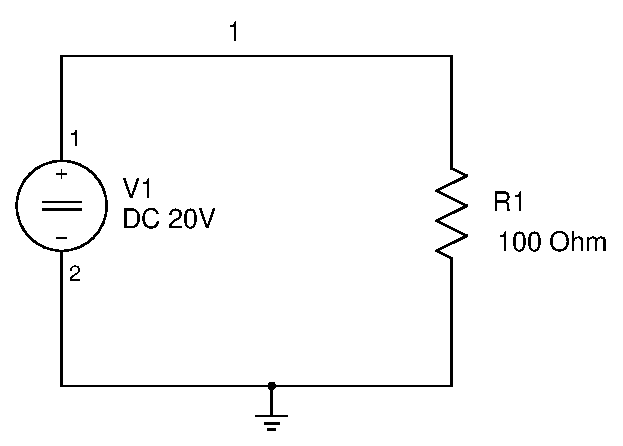
\includegraphics[scale=0.5]{img/voltage-resistor}
%\end{figure}
\end{center}


\vspace*{1in}

\begin{solution}
200 mA

\end{solution}

\end{questions}

\end{document}
